\chapter{Stiff string}\label{ch:stiffString}
Earlier, in Section \ref{sec:1DWave},the case of the ideal string was presented modelled using the 1D wave equation. As shown, the model generates an output with harmonic partials that are integer multiples of the fundamental frequency. In the real world, however, strings exhibit a phenomenon called \textit{inharmonicity} due to stiffness in the material. 

The restoring force of the 1D wave equation is only due to tension. In the real world, however, this force is also due to stiffness, dependent on the material and geometry of the string. This stiffness causes frequency dispersion and inharmonicity: the partials get exponentially further apart with frequency. 

The stiff string played a prominent part in many of the published works:
\citeP[A], \citeP[B], \citeP[C], \citeP[D] and \citeP[E]. 

This chapter will go into the PDE of the stiff string, and discretise it. The analysis techniques presented in the previous chapter will be applied to the stiff string. \todo{not done}

\section{Continuous time}
Consider a lossless \todo{should I even include the lossless one? It's just so that we can slowly build up to the damped model...}stiff string with a circular cross-section of length $L$. Its transverse displacement is described by $u=u(x,t)$ defined for $x\in \D$ with domain $\D = [0, L]$ and time $t\geq 0$. The PDE describing its motion is 
\begin{equation}\label{eq:stiffStringPDENoLosses}
    \rho A \ptt u = T \pxx u - EI \pxxxx u
\end{equation}
parameterised by material density $\rho$ (in kg/m$^3$), cross-sectional area $A = \pi r^2$ (in m$^2$), radius $r$ (in m) tension $T$ (in N), Young's modulus $E$ (in Pa) and area moment of inertia $I = \pi r^4/4$ (in m$^4$). If either $E$ or $I$ is 0, Eq \eqref{eq:stiffStringPDENoLosses} reduces to the 1D wave equation in Eq. \eqref{eq:1DwavePDE} where $c = \sqrt{T/\rho A}$. If instead $T = 0$, Eq. \eqref{eq:stiffStringPDENoLosses} reduces to the \textit{ideal bar} equation.


\subsubsection{Dispersion Analysis}
The 4th-order spatial derivative models \textit{frequency dispersion}, a phenomenon that causes different frequencies to travel at different speeds. As opposed to the undesired numerical dispersion 

\subsection{Adding Losses}
Before moving on to the discretisation of the PDE in \eqref{eq:stiffStringPDENoLosses}, losses can be added to the system. In the physical world, strings lose energy through fx. air viscosity and thermoelastic effects. All frequencies die out (damp) over time, but higher frequencies do so at a much faster rate. This phenomenon is called \textit{frequency-dependent damping} and can be modelled using a mixed derivative $\pt \pxx$. This way of frequency-dependent damping first appeared in \cite{Bensa2003} and has been used extensively in the literature since. The model of a damped stiff string is
\begin{equation}\label{eq:stiffStringPDE}
    \rho A \ptt u = T \pxx u - EI \pxxxx u - 2 \sz \rho A \pt u + 2 \so \rho A\pt \pxx u
\end{equation}
where the non-negative loss coefficients $\sz$ (in s$^{-1}$) and $\so$ (in m$^2$/s) determine the frequency dependent and frequency independent losses respectively. 

A more compact way to write Eq. \eqref{eq:stiffStringPDE}, and as is also found often in the literature \cite{theBible} \todo{etc.} is to divide both sides by $\rho A$ to get
\begin{equation}\label{eq:stiffStringPDECompact}
    \ptt u = c^2 \pxx u - \kappa^2 \pxxxx u - 2 \sz \pt u + 2 \so \pt \pxx u
\end{equation}
where $c=\sqrt{T/\rho A}$ is the wave speed \todo{check wavespeed or wave speed (entire document)} (in m/s) as in the 1D wave equation in \eqref{eq:1DwavePDE} and $\kappa = \sqrt{EI / \rho A}$ is a \textit{stiffness coefficient} (in m$^2$/s).

\subsubsection{Intuition}
Although Eq. \eqref{eq:stiffStringPDE} might look daunting at first, the principle of Newton's second law remains the same. 

Something about the 4th spatial derivative and the loss terms here...

\subsubsection{Boundary Conditions}
The boundary conditions found in Eq. \eqref{eq:boundaryCond1DWave} can be extended to
\begin{subequations}\label{eq:stiffStringBoundConds}
    \begin{align}
        u = \px u &= 0 \quad \text{(clamped)}\label{eq:BCclamped}\\
        u = \pxx u &= 0 \quad \text{(simply supported)}\label{eq:BCsimplySupported}\\
        \pxx u = \pxxx u &= 0 \quad \text{(free)}\label{eq:BCfree}
    \end{align}
\end{subequations}
at $x = 0, L$. See Figure \ref{fig:boundaryCondsStiffString} for plots of the first modal shape for each respective boundary condition. 
\def\figWidth{0.32}
\begin{figure}[h]
    \centering
    \subfloat[Clamped.\label{fig:clamped}]{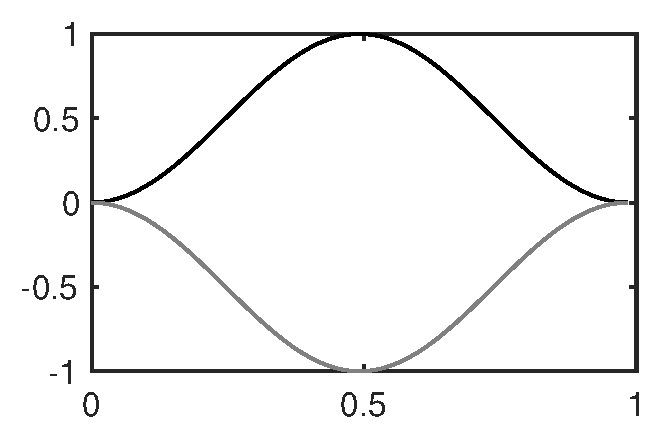
\includegraphics[width=\figWidth\textwidth]{figures/resonators/clamped.eps}}\hfill
    \subfloat[Simply supported.\label{fig:simplySupported}]{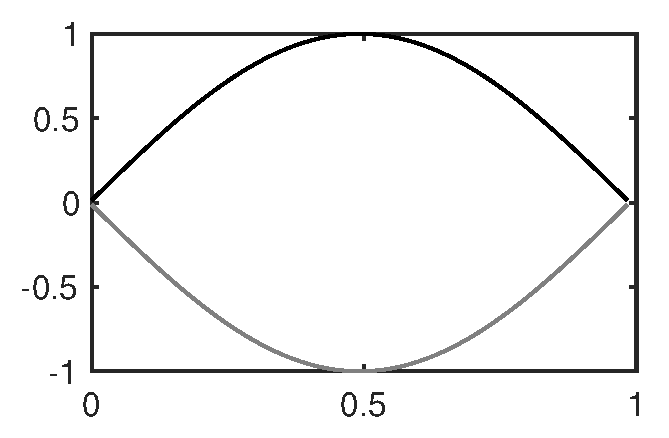
\includegraphics[width=\figWidth\textwidth]{figures/resonators/simplySupported.eps}}\hfill
    \subfloat[Free.\label{fig:free}]{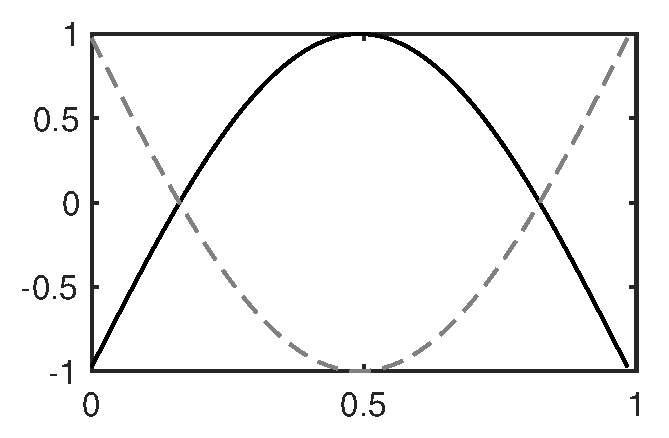
\includegraphics[width=\figWidth\textwidth]{figures/resonators/free.eps}}
    \caption{The first (normalised) modal shape for the three boundary conditions in Eqs. \eqref{eq:stiffStringBoundConds}. The extremes are indicated with black and grey lines respectively. \label{fig:boundaryCondsStiffString}}
\end{figure}

\section{Discrete Time}
For the sake of brevity we continue with Eq. \eqref{eq:stiffStringPDECompact}, rather than Eq. \eqref{eq:stiffStringPDE}. Naturally, same process can be followed for the latter, the only difference being a multiplication by $\rho A$ of all terms.

Equation \eqref{eq:stiffStringPDECompact} can be discretised as 
\begin{equation}\label{eq:stiffStringFDS}
    \dtt \uln = c^2 \dxx \uln - \kappa^2 \dxxxx \uln - 2 \sz \dtd \uln + 2 \so\dtm\dxx \uln,
\end{equation}
and is defined for domain $l\in\{0, \hdots, N\}$ and number of grid points $N+1$. 
The $\dxxxx$ operator is the second-order spatial difference in Eq. \eqref{eq:discSecondSpace} applied to itself
\begin{equation}\label{eq:dxxxx}
    \dxxxx = \dxx\dxx = \frac{1}{h^4}\left(e_{x+}^2 - 4e_{x+}+6 - 4e_{x-}+e_{x-}^2\right).
\end{equation} 
A multiplication of two shift operators applied to a grid function simply means to apply each shift individually. The $\dxxxx$ operator applied to $\uln$ thus becomes
\begin{equation}
    \dxxxx\uln = \frac{1}{h^4}\left(u_{l+2}^n - 4u_{l+1}^n+6\uln - 4u_{l-1}^n+u_{l-2}^n\right).
\end{equation}

A definition for the mixed-derivative operator can similarly be found.
Recalling the definitions for $\dtm$ in Eq. \eqref{eq:backwardTimeOperator} and $\dxx$ Eq. \eqref{eq:discSecondSpace}, their combination results in
\begin{align}
    \dtm\dxx &= \frac{1}{k}\left(1-e_{t-}\right)\frac{1}{h^2}\left(e_{x+}-2+e_{x-}\right),\nonumber \\
    &= \frac{1}{kh^2}\left(e_{x+}-2+e_{x-} - e_{t-}(e_{x+}-2+e_{x-})\right).
\end{align}
Two different shift operators multiplied together still simply means to apply them to the grid function individually. The $\dtm\dxx$ operator applied to $\uln$ thus yields
\begin{equation}
    \dtm \dxx \uln = \frac{1}{hk^2}\left(u_{l+1}^n - 2 \uln + u_{l-1}^n - u_{l+1}^{n-1} + 2 u_l^{n-1} - u_{l-1}^{n-1}\right).
\end{equation}
The reason a backwards difference is used here is to keep the system explicit. An example of an implicit scheme using the centred operator instead can be found in Section \ref{sec:implicitStiffString}.

With these definitions, 
the operators in scheme \eqref{eq:stiffStringFDS} can be expanded to get
\begin{equation}
    \begin{aligned}\label{eq:expandedStringFDS}
        \frac{1}{k^2}\big(u_l^{n+1} - 2\uln & + u_l^{n-1} \big) =\frac{c^2}{h^2}\left(u_{l+1}^n - 2\uln + u_{l-1}^n\right) \\
        &- \frac{\kappa^2}{h^4}\left(u_{l+2}^n - 4u_{l+1}^n+6\uln - 4u_{l-1}^n+u_{l-2}^n\right) \\ 
        &- \frac{\sz}{k} \left(u_l^{n+1} - u_l^{n-1}\right)\\
        & + \frac{2\so}{kh^2}\left(u_{l+1}^n - 2\uln + u_{l-1}^n - u_{l+1}^{n-1} + 2u_l^{n-1} + u_{l-1}^{n-1}\right),
    \end{aligned}
\end{equation}
and after multiplication by $k^2$ and collecting the terms yields
\begin{equation}
    \begin{aligned}
        (1+\sz k) u_l^{n+1} =&\ \left(2 - 2\lambda^2 - 6\mu^2 - \frac{4\so k}{h^2}\right) \uln\\
        & + \left(\lambda^2 + 4\mu^2 + \frac{2\so k}{h^2}\right) (u_{l+1}^n + u_{l-1}^n) \\
        &- \mu^2 (u_{l+2}^n + u_{l-2}^n) + \left(-1+\sz k + \frac{4\so k}{h^2}\right)u_l^{n-1}\\
        & - \frac{2\so k}{h^2}(u_{l+1}^{n-1} + u_{l-1}^{n-1}),
    \end{aligned}
\end{equation}
with 
\begin{equation}\label{eq:stiffStringCourant}
    \lambda = \frac{ck}{h} \qaq \mu = \frac{\kappa k}{h^2}.
\end{equation}
The update equation follows by dividing both sides by $(1+\sz k)$. 

The stability condition for the FD scheme in \eqref{eq:stiffStringFDS} is defined as 
\begin{equation}\label{eq:stiffStringStability}
    h \geq \sqrt{\frac{c^2k^2+4\so k + \sqrt{(c^2k^2 + 4\so k)^2+16\kappa^2k^2}}{2}},
\end{equation}
and will be derived in Section \ref{sec:stiffStringStability} using von Neumann analysis. 
This condition can then be used to calculate the number of intervals $N$ in a similar fashion as for the 1D wave equation shown in Eq. \eqref{eq:orderOfCalc}. First, Eq. \eqref{eq:stiffStringStability} should be satisfied with equality, after which
\begin{equation*}
    N := \floor[\frac{L}{h}], \qaq h := \frac{L}{N}
\end{equation*}
which can then be used to calculate $\lambda$ and $\mu$ in \eqref{eq:stiffStringCourant}.

\subsubsection{Stencil}
As done in Section \ref{sec:1DWaveDisc}, a stencil for the FD scheme implementing the damped stiff string can be created. This is shown in Figure \ref{fig:stencilStiffString}. In order to calculate $u_l^{n+1}$, $5$ points at the current time step are needed due to the 4\th-order spatial derivative. Due to the mixed derivative in the frequency-dependent damping term neighbouring points at the previous time step are also required. 
%, the coefficient multiplied onto $u_l^{n+1}$.

% and the terms collected to obtain the following update equation
% \begin{equation}
%     \begin{aligned}
%     % (1+\sz k) u_l^{n+1} =&\ \left(2 - 2\lambda^2 - 6\mu^2 - \frac{4\so k}{h^2}\right) \uln\\
%     % & + \left(\lambda^2 + 4\mu^2 + \frac{2\so k}{h^2}\right) (u_{l+1}^n + u_{l-1}^n) \\
%     % &- \mu^2 (u_{l+2}^n + u_{l-2}^n) + \left(-1+\sz k + \frac{4\sz k}{h^2}\right)u_l^{n-1}\\
%     % & - \frac{2\so k}{h^2}(u_{l+1}^{n-1} + u_{l-1}^{n-1})
%     % \end{aligned}
%     Au_l^{n+1} = &\ B_0 \uln + B_1 (u_{l+1}^n + u_{l-1}^n) + B_2 (u_{l+2}^n + u_{l-2}^n) \\
%     &+ C_0 u_l^{n-1} + C_1(u_{l+1}^{n-1} + u_{l-1}^{n-1}) 
%     \end{aligned}
% \end{equation}
% with coefficients
% \begin{gather*}
%     B_0 = 2 - 2\lambda^2 - 6\mu^2 - \frac{4\so k}{h^2}, \quad B_1 = \lambda^2 + 4\mu^2 + \frac{2\so k}{h^2}, \quad B_2 =- \mu^2, \\[1em]
%     C_0 =  -1+\sz k + \frac{4\so k}{h^2},\quad C_1 = - \frac{2\so k}{h^2}, \qaq A = 1+\sz k.
% \end{gather*}
% Note that for clarity the division by $A$ has been left for implementation. 
\begin{figure}[h]
    \centering
    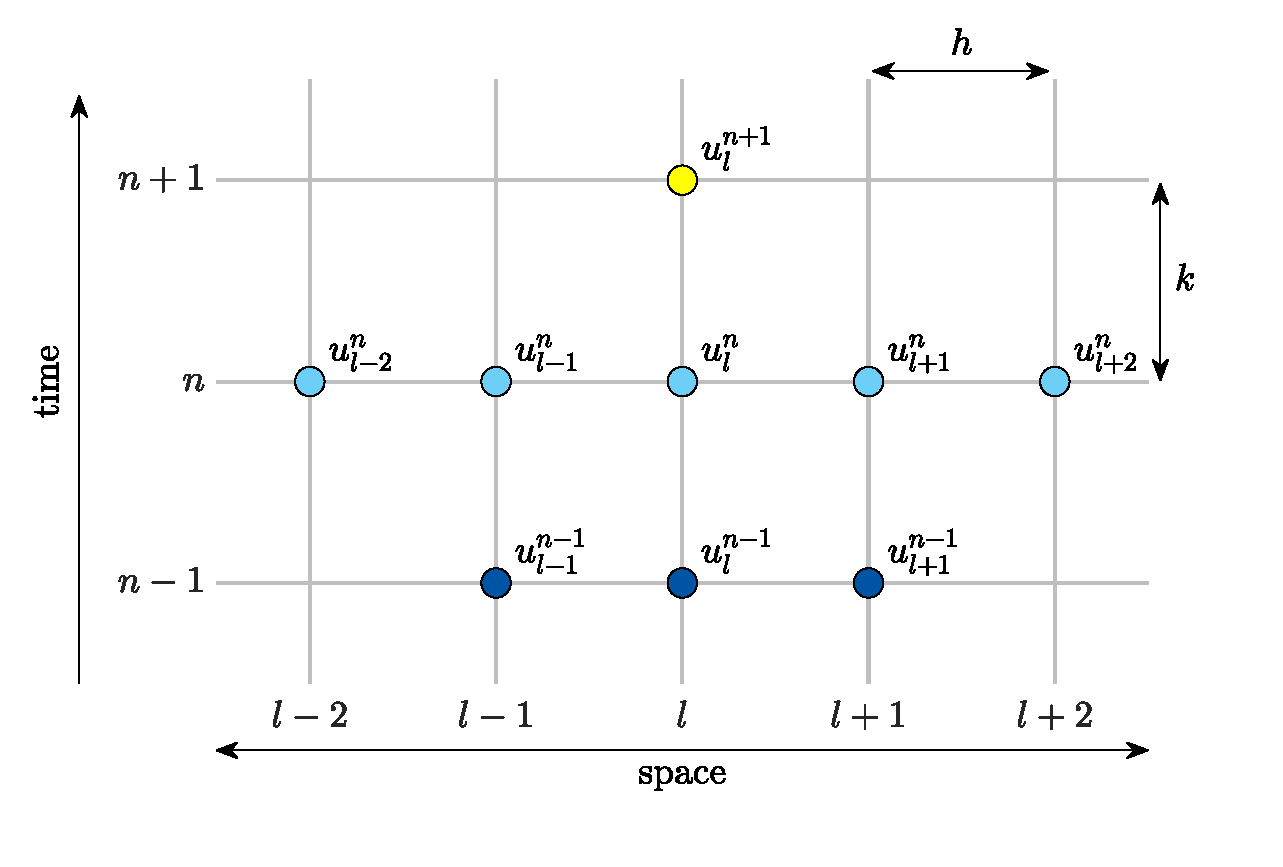
\includegraphics[width=0.8\textwidth]{figures/resonators/stencilDampedStiffString.eps}
    \caption{The stencil for the damped stiff string scheme in \eqref{eq:stiffStringFDS}.\label{fig:stencilStiffString}}
\end{figure}

\subsection{Boundary conditions}
Due to the 4\th-order spatial derivative, two virtual grid points need to be accounted for at the boundaries of the system. Discretising the boundary conditions in \eqref{eq:stiffStringBoundConds} yields
\begin{subequations}\label{eq:stiffStringBoundCondsDisc}
    \begin{align}
        \uln = \delta_{x\pm} \uln &= 0 \quad \text{(clamped)}\label{eq:BCclampedDisc}\\
        \uln = \dxx \uln &= 0 \quad \text{(simply supported)}\label{eq:BCsimplySupportedDisc}\\
        \dxx \uln = \dxd\dxx \uln &= 0 \quad \text{(free)}\label{eq:BCfreeDisc}
    \end{align}
\end{subequations}
at $l = 0, N$. The operator in the clamped condition uses the $\dxp$ operator at the left boundary ($l = 0$) and $\dxm$ at the right ($l = N$). Note that for the free boundary condition, to discretise $\px^3$ in Eq. \eqref{eq:BCfree} the less accurate $\dtm \dxx$ and $\dtp \dxx$ operators could be chosen for the left and right boundary respectively. Here, however, we use the most accurate option $\dxd\dxx$. 

Below, the boundary conditions are solved and update equations at the boundaries are given.

\todo{insert figure showing virtual grid points somewhere in this section}

\subsubsection{Clamped}
Expanding the operators for the clamped condition yields 
\begin{equation}
    u_0^n = u_1^n = 0 \qaq u_{N-1}^n = u_N^n = 0.
\end{equation}
This can be simplified by reducing the range of calculation to $l\in \{ 2, \hdots, N-2\}$.

\subsubsection{Simply supported}
As the states of the end points of a system with simply supported boundary conditions are $0$ at all times, the range of calculation can be reduced to $l\in \{ 1, \hdots, N-1\}$. At $l=1$ and $l=N-1$ the virtual grid points $u_{-1}^n$ and $u_{N+1}^n$ are needed. A definition for $u_{-1}^n$ can be found by expanding Eq. \eqref{eq:BCsimplySupportedDisc} at $l = 0$:
\begin{align}
    &\frac{1}{h^2}\left(u_1^n - 2 u_0^n + u_{-1}^n\right) = 0,\nonumber\\[-1em]
    \xLeftrightarrow{\mystrut\ u^n_0 = 0\ } \quad & u_1^n + u_{-1}^n = 0,\nonumber\\[0.25em]
    &u_{-1}^n = -u_1^n,\label{eq:simplySupportedResult}
\end{align}
and similarly for $u_{N+1}^n$ by expanding the condition at $l=N$:
\begin{equation*}
    u_{N+1}^n = -u_{N-1}^n.
\end{equation*}
Filling these definitions into the expanded scheme at $l=1$ in \eqref{eq:expandedStringFDS} and collecting the terms yields
\begin{equation}
    \begin{aligned}
        \!\!\!\!\!(1+\sz k) u_1^{n+1} =&\ \left(2 - 2\lambda^2 - 5\mu^2 - \frac{4\so k}{h^2}\right) u_1^n + \left(\lambda^2 + 4\mu^2 + \frac{2\so k}{h^2}\right) u_{2}^n \\
        &-\mu^2u_3^n+ \left(-1+\sz k + \frac{4\sz k}{h^2}\right)u_1^{n-1} - \frac{2\so k}{h^2}u_{2}^{n-1}.
    \end{aligned}
\end{equation}
Doing the same for $l=N-1$:
\begin{equation}
    \begin{aligned}
        \!\!\!\!\!(1+\sz k) u_{N-1}^{n+1} =&\ \left(2 - 2\lambda^2 - 5\mu^2 - \frac{4\so k}{h^2}\right) u_{N-1}^n + \left(\lambda^2 + 4\mu^2 + \frac{2\so k}{h^2}\right) u_{N-2}^n \\
        &-\mu^2u_{N-3}^n+ \left(-1+\sz k + \frac{4\sz k}{h^2}\right)u_{N-1}^{n-1} - \frac{2\so k}{h^2}u_{N-2}^{n-1}.
    \end{aligned}
\end{equation}

\subsubsection{Free}
Finally, the free boundary condition requires all points to be calculated and $l\in\{0, \hdots, N\}$. 
The combined operator in Eq. \eqref{eq:BCfreeDisc} is defined as:
\begin{align}
    \dxd\dxx &= \frac{1}{2h^3}\left(e_{x+}-e_{x-}\right)\left(e_{x+}-2+e_{x-}\right),\nonumber\\
    &=\frac{1}{2h^3}\left(e_{x+}^2 - 2e_{x+} + 1 - (1 - 2e_{x-} + e_{x-}^2\right),\nonumber\\
    &=\frac{1}{2h^3}\left(e_{x+}^2 - 2e_{x+} + 2e_{x-} -e_{x-}^2\right).
\end{align}
This can be used to solve for the virtual grid points in the free condition at $l=0$:
\begin{align*}
    \frac{1}{2h^3} &\left(u_2^n - 2 u_1^n + 2u_{-1}^n - u_{-2}^n\right) = 0,\\%[0.25em]
    u_{-2}^n &= u_2^n - 2 u_1^n + 2u_{-1}^n.
    % \\[-1em]
    % \!\!\!\!\!\!\!\!\!\!\!\!\!\!\!\xLeftrightarrow{\mystrut\ \dxx \uln = 0\ \Rightarrow\ \text{ Eq. \eqref{eq:simplySupportedResult}}\ }
    % \quad u_{-2}^n &= u_2^n - 4 u_1^n 
\end{align*}
As $u_0^n$ is not necessarily $0$ at all times, solving the first part of the boundary condition yields a different result than in the simply supported case:
\begin{align*}
    \frac{1}{h^2} &\left(u_1^n - 2 u_0^n + u_{-1}^n \right) = 0,\\
    u_{-1}^n &= 2u_0^n - u_1^n.
    % \\[-1em]
    % \!\!\!\!\!\!\!\!\!\!\!\!\!\!\!\xLeftrightarrow{\mystrut\ \dxx \uln = 0\ \Rightarrow\ \text{ Eq. \eqref{eq:simplySupportedResult}}\ }
    % \quad u_{-2}^n &= u_2^n - 4 u_1^n 
\end{align*}
The same can be done at $l=N$ to get
\begin{equation*}
    u_{N+2}^n = u_{N-2}^n - 2 u_{N-1}^n + 2u_{N+1}^n
    \qaq u_{N+1}^n = 2u_N^n - u_{N-1}^n.
\end{equation*}
The update equations for the boundary points will not be given here. Instead the form of the matrices will be provided below. 
% The update equation at $l=0$ then becomes
% \begin{equation}
%     \begin{aligned}
%         \!\!\!\!\!(1+\sz k) u_0^{n+1} =&\ \left(2 - 2\lambda^2 - 2 \mu^2 - \frac{4\so k}{h^2}\right) u_0^n + \left(\lambda^2 +4\mu^2 + \frac{4\so k}{h^2}\right) u_1^n \\
%         &-2\mu^2u_2^n+ \left(-1+\sz k + \frac{4\sz k}{h^2}\right)u_0^{n-1} - \frac{4\so k}{h^2}u_1^{n-1}.
%     \end{aligned}
% \end{equation}
% at $l=1$
% \begin{equation}
%     \begin{aligned}
%         \!\!\!\!\!(1+\sz k) u_1^{n+1} =&\ \left(2 - 2\lambda^2 - 5\mu^2 - \frac{4\so k}{h^2}\right) u_1^n + \left(\lambda^2 + 4\mu^2 + \frac{2\so k}{h^2}\right) u_{2}^n \\
%         &-2\mu^2u_3^n+ \left(-1+\sz k + \frac{4\sz k}{h^2}\right)u_1^{n-1} - \frac{2\so k}{h^2}u_{2}^{n-1}.
%     \end{aligned}
% \end{equation}

In practice, the simply supported boundary condition is mostly chosen as this reflects reality most. The clamped condition could be chosen for simplicity as this does not require an alternative update at the boundaries. The free boundary condition is more often used to model a (damped) ideal bar, (Eq. \eqref{eq:stiffStringPDE} with $T = 0$).

\subsection{Implementation and Matrix Form}
When using \texttt{MATLAB}, to prevent clutter in the code, it is useful to write the scheme in matrix form. The FD scheme of the stiff string in \eqref{eq:stiffStringFDS} can be written as 
\begin{equation}\label{eq:matrixFormStiffStringImplicit}
    A\u^{n+1} = \B\u^n + \C \u^{n-1}
\end{equation}
where 
\begin{equation}
    \begin{gathered}
    A = (1+\sz k), \quad \B = c^2 k^2 \Dxx - \kappa^2 k^2 \Dxxxx + 2 \so k \Dxx \\
    \text{and} \quad \C = -(1-\sz k)\I - 2\so k \Dxx.
    \end{gathered}
\end{equation}
Notice that $A$ is a scalar rather than a matrix.

The size of the state vectors and the matrix-form operators depend on the boundary conditions. For clamped conditions the state vectors ($\u^{n+1}$, $\u^n$ and $\u^{n-1}$) and matrices will be of size $(N-3) \times 1$ and $(N-3) \times (N-3)$ respectively. The $\Dxx$ matrix will be of the form given in \eqref{eq:DxxDef} and the matrix form of the $\dxxxx$ operator is
\begin{equation}
    \mathbf{D}_{xxxx} = \frac{1}{h^4}\begin{bmatrix}
        6& -4 & 1 & & \mathbf{0} \\
        -4 & 6 &\ddots &\ddots & \\
        1& \ddots & \ddots & \ddots&1 \\
        &\ddots & \ddots & 6 & -4 \\
        \mathbf{0} & & 1& -4 & 6 \\
    \end{bmatrix}.
\end{equation}

For simply supported conditions, the state vectors and matrices will be of size $(N-1) \times 1$ and $(N-1) \times (N-1)$ respectively. Again, $\Dxx$ is as defined in \eqref{eq:DxxDef} and $\Dxxxx$ can be obtained by multiplying two $\Dxx$ matrices according to 
\begin{equation}
    \Dxx\Dxx = \mathbf{D}_{xxxx} = \frac{1}{h^4}\begin{bmatrix}
        5& -4 & 1 & & & \mathbf{0}& \\
        -4 & 6 &\ddots &\ddots & & & \\
        1& \ddots & \ddots & -4 & 1 & & \\
        & \ddots& -4 & 6 & -4 & \ddots& \\
        & & 1 & -4 & \ddots & \ddots &1 \\
        & & & \ddots & \ddots & 6 & -4 \\
        & \mathbf{0} & & & 1& -4 & 5 \\
    \end{bmatrix}.
\end{equation}

Finally for free boundary conditions as given in \eqref{eq:BCfreeDisc}, the state vectors and matrices are $(N+1)\times 1$ and $(N+1)\times (N+1)$ respectively. Now, the $\Dxx$ matrix is of the form in \eqref{eq:DxxDefNeumann} and

\setstackgap{L}{16pt}
\setstacktabbedgap{8pt}
\def\lrgap{\kern3pt}
\fixTABwidth{T}
\begin{equation}
    \mathbf{D}_{xxxx} = \frac{1}{h^4}\xbracketMatrixstack{
        2& -4 & 2 & & & \mathbf{0}& \\
        -2 & 5 & -4 & 1 & & & \\
        1& -4 & 6 & -4 & 1 & & \\
        & \ddots & \ddots & \ddots & \ddots &\ddots & \\
        & & 1 & -4 & 6 & -4 &1 \\
        & & & 1 & -4 & 5 & -2 \\
        & \mathbf{0} & & & 2& -4 & 2}.
\end{equation}


\section{von Neumann Analysis and Stability Condition}\label{sec:stiffStringStability}
In order to obtain the stability condition for the damped stiff string, one can perform von Neumann analysis as presented in Section \ref{sec:stabilityAnalysis} on scheme \eqref{eq:stiffStringFDS}.

Using the definitions found in Eq. \eqref{eq:temporalAnsatz} for the temporal operators and Eqs. \eqref{eq:dxxAnsatz} and \eqref{eq:dxxxxAnsatz} for the spatial operators, the frequency-domain representation of Eq. \eqref{eq:stiffStringFDS} can be obtained:
\begin{align*}
    \!\!\!\!\frac{1}{k^2}\left(z - 2 + z^{-1}\right) =&-\frac{4c^2}{h^2}\sin^2(\beta h/2) - \frac{16\kappa^2}{h^4}\sin^4(\beta h/2) - \frac{\sz}{k}z + \frac{\sz}{k}z^{-1}\\
    & - \frac{8 \so}{kh^2}\sin^2(\beta h/2) + \frac{8 \so}{kh^2} \sin^2(\beta h/2)z^{-1}
\end{align*}
and after collecting the terms, the characteristic equation follows
\begin{gather}
    (1+\sz k)z + \left(16\mu^2\sin^4(\beta h/2)+\left(4\lambda^2+\frac{8\so k}{h^2}\right)\sin^2(\beta h/2) - 2\right)\nonumber\\
    +\left(1-\sz k-\frac{8\so k}{h^2}\sin^2(\beta h/2)\right)z^{-1}=0.\label{eq:charDampedString}
\end{gather}
Rewriting this to the form \eqref{eq:polynomialForm}, and using $\S = \sin^2(\beta h /2)$ for brevity, yields
\begin{equation*}
    z^2 + \left(\frac{16\mu^2\S^2+\left(4\lambda^2+\frac{8\so k}{h^2}\right)\S - 2}{1 + \sz k}\right)z+\frac{1-\sz k-\frac{8\so k}{h^2}\S}{1 + \sz k}=0.
\end{equation*}
Stability of the system can then be proven using condition \eqref{eq:condition214}. Substituting the coefficients into this condition yields
\begin{equation}\nonumber
    \begin{aligned}
        \left|\frac{16\mu^2\S^2+\left(4\lambda^2+\frac{8\so k}{h^2}\right)\S - 2}{1+\sz k}\right|-1 &\leq \frac{1-\sz k-\frac{8\so k}{h^2}\S}{1+\sz k}\leq 1,\\
        \left|16\mu^2\S^2+\left(4\lambda^2+\frac{8\so k}{h^2}\right)\S - 2\right|-(1+\sz k) &\leq 1-\sz k-\frac{8\so k}{h^2}\S\leq 1+\sz k,\\
        \left|16\mu^2\S^2+\left(4\lambda^2+\frac{8\so k}{h^2}\right)\S - 2\right|&\leq2-\frac{8\so k}{h^2}\S\leq2+2\sz k.
    \end{aligned}
\end{equation}
The second condition is always true due to the fact that $\sigma_0,\sigma_1 \geq 0$. Continuing with the first condition: 
\begin{align*}
    -2+\frac{8\so k}{h^2}\S&\leq 16\mu^2\S^2+\left(4\lambda^2+\frac{8\so k}{h^2}\right)\S - 2\leq 2-\frac{8\so k}{h^2}\S,\\
    0&\leq 16\mu^2\S^2+4\lambda^2\S\leq 4-\frac{16\so k}{h^2}\S.
\end{align*}
As $16\mu^2\S^2+4\lambda^2\S$ is positive definite, the first condition is always satisfied. Continuing with the second condition:
\begin{align*}
    16\mu^2\S^2+\left(4\lambda^2+ \frac{16\so k}{h^2}\right)\S &\leq 4,\\
    4\mu^2\S^2+\left(\lambda^2+ \frac{4\so k}{h^2}\right)\S&\leq 1.
\end{align*}
As $\S$ is bounded by $1$, this can be substituted as it challenges the condition the most. \todo{different wording} Continuing with the substituted definitions for $\lambda$ and $\mu$ from Eq. \eqref{eq:stiffStringCourant} yields
\begin{align*}
    \frac{4\kappa^2k^2}{h^4}+\frac{c^2k^2 + 4\so k}{h^2}&\leq 1, \\
    4\kappa^2k^2+(c^2k^2+ 4\so k)h^2&\leq h^4,\\
    h^4- (c^2k^2+ 4\so k)h^2 - 4\kappa^2k^2 &\geq 0 ,
\end{align*}
which is a quadratic equation in $h^2$ with $h$ bounded by
\begin{equation}
    h \geq \sqrt{\frac{c^2k^2+4\so k + \sqrt{(c^2k^2 + 4\so k)^2+16\kappa^2k^2}}{2}}.
\end{equation}
This is the stability condition for the damped stiff string also shown in Eq. \eqref{eq:stiffStringStability}.

\section{Energy Analysis}\label{sec:energyAnalysisString}
As mentioned in Section \ref{sec:energyAnalysis}, it is useful to perform the energy analysis on the scheme with all physical parameters written out. Discretising PDE \eqref{eq:stiffStringPDE} yields
\begin{equation}
    \rho A \dtt \uln = T \dxx \uln - EI \dxxxx \uln - 2\sz \rho A \dtd \uln + 2 \so \rho A \dtm \dxx \uln,
\end{equation}
defined for $l\in d$ with discrete domain $d = \{0, \hdots, N\}$. This section will follow the 4 steps described in Section \ref{sec:energyAnalysis}.

\subsubsection{Step 1: Obtain $\dtp \h$}
The first step is to take the inner product of the scheme with $(\dtd \uln)$ over discrete domain $d$
\begin{equation}\label{eq:rOCStiffString}
    \begin{aligned}
    \dtp \h =&\ \rho A \langle \dtd \uln, \dtt \uln \rangle_d - T \langle \dtd \uln, \dxx \uln\rangle_d + EI \langle \dtd \uln, \dxxxx \uln \rangle_d\\
    & + 2\sz\rho A \langle \dtd \uln, \dtd \uln \rangle_d - 2\so \rho A\langle \dtd \uln, \dtm \dxx \uln \rangle_d = 0.
    \end{aligned}
\end{equation}  


\subsubsection{Step 2: Identify energy types and isolate $\dtp$}
As there is damping present in the system, and the system is distributed, the energy balance will be of the form 
\begin{equation}
    \dtp \h = \mathfrak{b}-\mathfrak{q},
\end{equation}
where the boundary term $\mathfrak{b}$ appears after summation by parts shown shortly, and
\begin{equation}\label{eq:dampingTermStiffString}
    \mathfrak{q} = 2\sz \rho A \lVert\dtd\uln\rVert_d^2 - 2 \so \rho A \langle \dtd \uln, \dtm \dxx \uln \rangle_d.
\end{equation}
Equation \eqref{eq:rOCStiffString} can be rewritten using summation by parts (see Section \ref{sec:summationByParts}). Specifically, using Eq. \eqref{eq:summationByPartsMinusBar} for the second term and Eq. \eqref{eq:summationByPartsTwiceReduced} for the third, we get
\begin{equation*}
    \dtp \h = \rho A \langle \dtd \uln, \dtt \uln \rangle_d + T \langle \dtd \dxp \uln, \dxp \uln\rangle_{\underline{d}} + EI \langle \dtd \dxx \uln, \dxx \uln \rangle_{\overline{\underline{d}}} = \mathfrak{b} - \mathfrak{q}
\end{equation*}
where the boundary term becomes
\begin{align*}
    \mathfrak{b} =&\ T\Big((\dtd u_N^n)(\dxp u_N^n) - (\dtd u_0^n) (\dxp u_{-1}^n)\Big) \\
    &+ EI \Big((\dtd u_N^n)(\dxp \dxx u_N^n) - (\dxx u_N^n)(\dxm \dtd u_N^n) \Big)\\
    &+ EI \Big(- (\dtd u_0^n)(\dxm \dxx u_0^n) + (\dxx u_0^n)(\dxp \dtd u_0^n)\Big).
\end{align*}
For the clamped and simply supported boundary conditions in \eqref{eq:BCclampedDisc} and \eqref{eq:BCsimplySupportedDisc} it can easily be shown that $\mathfrak{b} = 0$. For the boundary conditions to vanish when using the the free condition in 
\eqref{eq:BCfreeDisc}, the primed inner product and identity \eqref{eq:summationByPartsTwicePrimed} should be used. Here we continue with the unprimed inner product.

Isolating $\dtp$ to obtain the total energy $\h$ in the definition for $\dtp \h$ above, requires identities \eqref{eq:prodIdentity1} and \eqref{eq:prodIdentity2} and yields
\begin{equation*}
    \begin{aligned}
        \dtp\h &= \dtp\left(\frac{\rho A}{2}\lVert\dtm \uln\rVert_d^2 + \frac{T}{2}\langle\dxp\uln, e_{t-}\dxp\uln\rangle_{\underline{d}} + \frac{EI}{2}\langle\dxx\uln, e_{t-}\dxx\uln\rangle_{\overline{\underline{d}}}\right) \\
        &=-\mathfrak{q}.
    \end{aligned}
\end{equation*}
From this, the definition for the Hamiltonian $\h$, the kinetic energy $\t$ and potential energy $\v$ can be found:
\begin{equation}\label{eq:energyBalanceStiffString}
    \begin{gathered}
        \h = \t + \v, \qwiq \t = \frac{\rho A}{2}\lVert\dtm \uln\rVert^2_d,\text{and} \\
        \v = \frac{T}{2}\langle\dxp\uln, e_{t-}\dxp\uln\rangle_{\underline{d}} + \frac{EI}{2}\langle\dxx\uln, e_{t-}\dxx\uln\rangle_{\overline{\underline{d}}}.
    \end{gathered}
\end{equation}

\subsubsection{Step 3: Check units}
Comparing the energy balance in Eq. \eqref{eq:energyBalanceStiffString} to Eq. \eqref{eq:energyBalance1DWave}, one can observe that apart from the second term in the definition for $\v$ in the latter, the balances are identical. 
Writing this term out in units, and recalling that Pa (the unit for $E$) in SI units is kg$\cdot$m$^{-1}\cdot$s$^{-2}$, yields
\begin{align*}
    \frac{EI}{2}\langle\dxx\uln, e_{t-}\dxx\uln\rangle_{\overline{\underline{d}}}\overset{\text{in units}}{\xrightarrow{\hspace*{1cm}}}& \ \text{Pa}\cdot \text{m}^4 \cdot \text{m} \cdot (\text{m}^{-2} \cdot \text{m} \cdot \text{m}^{-2} \cdot \text{m}) \\
    & = \text{kg} \cdot \text{m}^2 \cdot \text{s}^{-2},
\end{align*}
and has indeed the correct units. 

The damping terms in $\mathfrak{q}$ need to be in Joules per second, or kg $\cdot$ m$^2 \cdot$ s$^{-3}$. Writing the terms in Eq. \eqref{eq:dampingTermStiffString} out in their units yields
\begin{align*}
    2\sz \rho A \lVert\dtd\uln\rVert_d^2\overset{\text{in units}}{\xrightarrow{\hspace*{1cm}}}&\ \text{s}^{-1}\cdot\text{kg}\cdot\text{m}^{-3}\cdot\text{m}^2\cdot \text{m}\cdot(\text{s}^{-1}\cdot\text{m})^2 \\
    &= \text{kg} \cdot \text{m}^2 \cdot \text{s}^{-3},\\
    - 2 \so \rho A \langle \dtd \uln, \dtm \dxx \uln \rangle_d \overset{\text{in units}}{\xrightarrow{\hspace*{1cm}}}&\  \text{m}^2\cdot\text{s}^{-1}\cdot\text{kg}\cdot\text{m}^{-3}\cdot\text{m}^2\\
    &\cdot\text{m}\cdot(\text{s}^{-1}\cdot\text{m})(\text{s}^{-1}\cdot\text{m}^{-2}\cdot \text{m}),\\
    &= \text{kg} \cdot \text{m}^2 \cdot \text{s}^{-3}
\end{align*}

\subsubsection{Step 4: Implementation}
Matrix form...

\section{Modal analysis}
To perform a modal analysis on the FD scheme of the damped stiff string in \eqref{eq:stiffStringFDS} 




\section{Implicit scheme}\label{sec:implicitStiffString}
Although not used in the published work of this project, I would like to touch upon an example of an implicit scheme. Consider a discretisation of Eq. \eqref{eq:stiffStringPDECompact} where the (more accurate) centred operator is used for the frequency-dependent damping term:
\begin{equation}\label{eq:stiffStringFDSImplicit}
    \dtt \uln = c^2 \dxx \uln - \kappa^2 \dxxxx \uln - 2 \sz \dtd \uln + 2 \so\dtd\dxx \uln.
\end{equation}
Using the centred operator in the mixed-spatial-temporal operator renders the system implicit, meaning that a definition for $u_l^{n+1}$ can not explicitly be found. The stencil in Figure \ref{fig:stencilStiffStringImplicit} also shows this: in order to calculate $u_l^{n+1}$, neighbouring points at the next time step $u_{l+1}^{n+1}$ and $u_{l-1}^{n+1}$ are needed. The issue is that these values are unknown at the time of calculation.

Luckily, as the scheme is linear, it can be treated as a system of linear equations and solved following the technique described in Section \ref{sec:linearEquations}. The drawback is that this requires one matrix inversion per iteration which can be extremely costly (see Section \ref{sec:RTmatrixInversion}). However, both von Neumann and modal analysis (below) show that using the centred instead of the backwards operator has a positive effect on the stability and the modal behaviour of the scheme. 

taking simply supported boundary conditions such that $l \in \{1, \hdots, N-1\}$ are $N-1$ unknowns that can be calculated using $N-1$ equations. The column vector $\u^n = [u_1^n, u_2^n, \hdots, u_{N-1}^n]$

\begin{equation}\label{eq:matrixFormStiffStringImplicit}
    \A\u^{n+1} = \B\u^n + \C \u^{n-1}
\end{equation}

\begin{figure}[h]
    \centering
    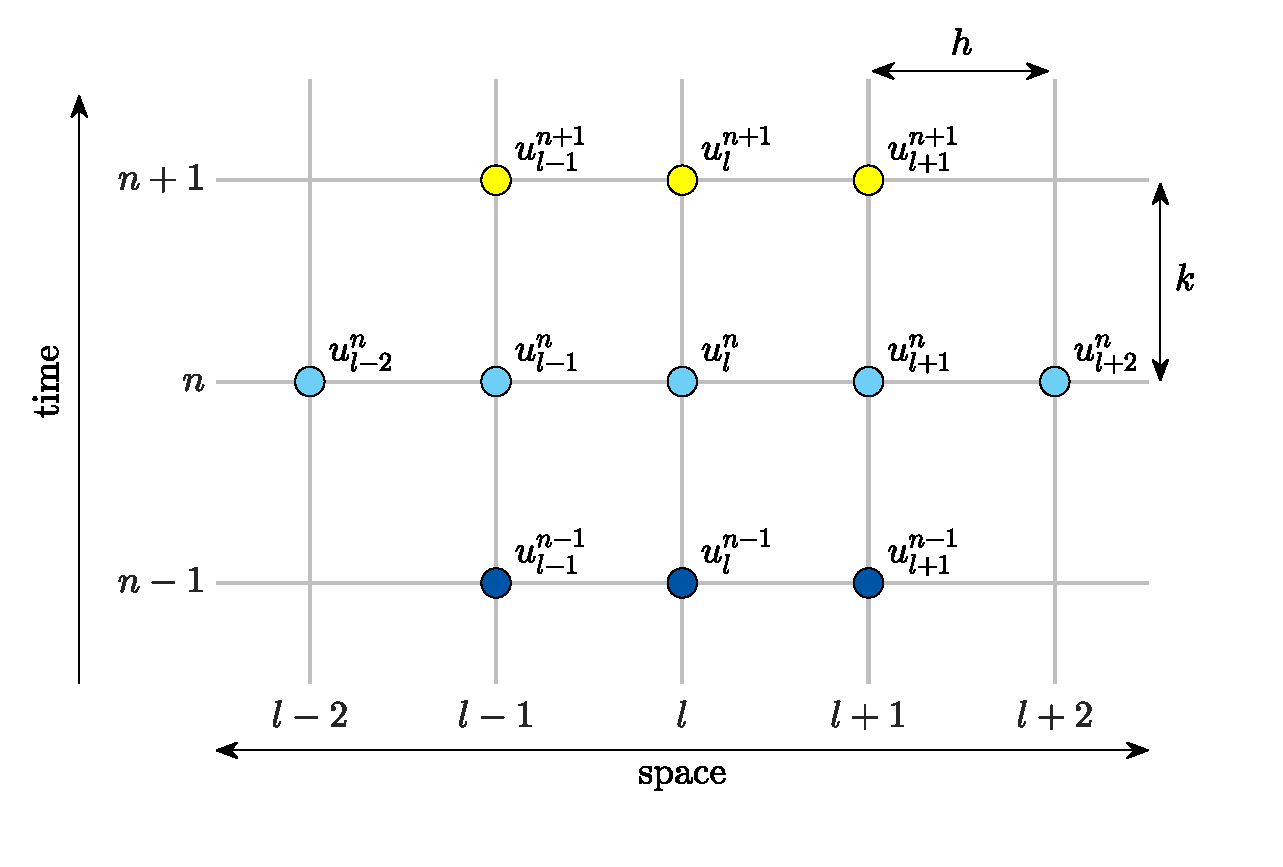
\includegraphics[width=0.8\textwidth]{figures/resonators/stencilImplicitStiffString.eps}
    \caption{The stencil for the damped stiff string scheme in \eqref{eq:stiffStringFDSImplicit}.\label{fig:stencilStiffStringImplicit}}
\end{figure}

\subsection{von Neumann analysis}
Following Section \ref{sec:stabilityAnalysis}..
\todo{below is the exact same wording as above}
\begin{align}
    \!\!\!\!\frac{1}{k^2}\left(z - 2 + z^{-1}\right) =&-\frac{4c^2}{h^2}\sin^2(\beta h/2) - \frac{16\kappa^2}{h^4}\sin^4(\beta h/2) - \sz kz + \sz k z^{-1}\nonumber\\
    & - \frac{4 \so  k}{h^2}\sin^2(\beta h/2)z + \frac{4 \so  k}{h^2} \sin^2(\beta h/2)z^{-1}
\end{align}
and after collecting the terms, the characteristic equation follows
\begin{gather}
\left(1+\sz k + \frac{4\so k}{h^2}\sin^2(\beta h/2)\right)z + \left(16\mu^2\sin^4(\beta h/2)+4\lambda^2\sin^2(\beta h/2) - 2\right)\nonumber\\
+ \left(1-\sz k - \frac{4\so k}{h^2}\sin^2(\beta h/2)\right)z^{-1} = 0.\label{eq:charDampedStiffSTring}
\end{gather}
Rewriting this to the form \eqref{eq:polynomialForm} and, again, using $\S = \sin^2(\beta h / 2)$ yields:
\begin{equation*}
z^2 + \frac{16\mu^2\S^2+4\lambda^2\S - 2}{1+\sz k + \frac{4\so k}{h^2}\S}z+\frac{1-\sz k - \frac{4\so k}{h^2}\S}{1+\sz k + \frac{4\so k}{h^2}\S} = 0.
\end{equation*}
stability of the system can be proven using condition \eqref{eq:condition214}. Continuing with $\S = \sin^2(\beta h/2)$ and substituting the coefficients into this condition yields
\begin{align*}
\left|\frac{16\mu^2\S^2+4\lambda^2\S - 2}{1+\sz k + \frac{4\so k}{h^2}\S} \right|-1 &\leq \frac{1-\sz k - \frac{4\so k}{h^2}\S}{1+\sz k + \frac{4\so k}{h^2}\S}\leq 1,\\[1em]
\left|16\mu^2\S^2+4\lambda^2\S - 2 \right| - \left(1+\sz k + \frac{4\so k}{h^2}\S\right) &\leq 1-\sz k - \frac{4\so k}{h^2}\S\\
&\leq 1+\sz k + \frac{4\so k}{h^2}\S,\\[1em]
\left|16\mu^2\S^2+4\lambda^2\S - 2 \right|&\leq 2 \leq 2+2\sz k + \frac{8\so k}{h^2}\S
\end{align*} 
Because $\sz, \so, k, \S$ and $h$ are all non-negative, the last condition is always satisfied. Continuing with the first condition:

\subsection{Modal analysis}
As Eq. \eqref{eq:matrixFormStiffStringImplicit} matches the form in Eq. \eqref{eq:modalForm}, one can perform a modal analysis by writing the scheme in one-step form as explained in Section \ref{sec:oneStepForm}